\chapter{Model Based Performance Testing}

\section{System Under Test}
The system that is modeled for performance testing is a middleware based distributed system which can be depicted in three layers as shown in Figure\ref{fig:systemfigure}.

\begin{figure}
 \centering
 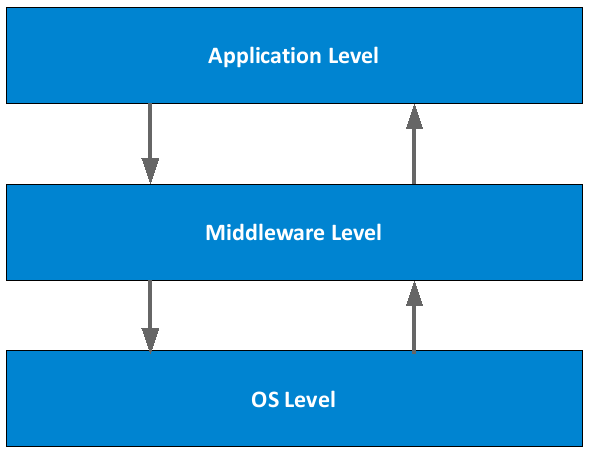
\includegraphics[width=0.8\textwidth]{figures/SystemFigure.png}
 % SystemFigure.png: 1179666x1179666 pixel, 0dpi, infxinf cm, bb=
 \caption{System Architecture}
 \label{fig:systemfigure}
\end{figure}

The modeled system is based on the XDAQ framework which is developed at CERN as a platform for the development of distributed data acquisition system \cite{CMSTDR}. A brief background on CMS XDAQ system is given in Chapter \ref{Chapter:DAQ}

!!!WRITE MORE ABOUT XDAQ AND CMS!!!

\subsection{Application Layer}
There are four applications that exist in the application level. Those are Event Manager (EVM), Readout Unit (RU), Builder Unit (BU), and Peer Transport (PT).

Peer Transports are special applications that carry out the data transmission in the distributed programming environment. Data transmission in XDAQ and Peer Transports are explained in detail in the CMS DAQ Technical Design Report \cite{CMSTDR}. 

EVM, RU and BU applications form the RU Builder which is part of a larger system called the event builder (EVB). Given the distributed nature of the EVB, it is responsible with reading event fragments from one set of nodes and assembling them into entire events on another set of nodes. Figure \ref{fig:evbsystem} shows the event builder and how the RU Builder is connected to the rest of the system \cite{rubuilder}. 

\begin{figure}
	\centering
		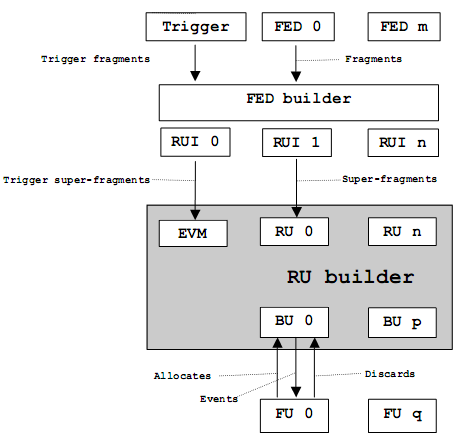
\includegraphics[width=0.90\textwidth]{figures/evbsystem.png}
	\caption{RU Builder Connected to Event Builder}
	\label{fig:evbsystem}
\end{figure}

This research is interested in the RU Builder and the applications that make up the RU Builder. Details of all the other components are given in \cite{CMSTDR}.

Event Manager (EVM) is the component which is responsible for determining the data flow in the RU Builder. Mainly, EVM assigns event id's to the events coming into the RU Builder. In addition, EVM manages the lifetime of the event id's as long as they are in the RU Builder. For this reason, EVM is the only component that knows about the status of the assigned event id's being processed in the RU Builder. EVM is in communication with all the RUs and BUs in the RU Builder \cite{CMSTDR}.

Readout Unit (RU) is the component which is responsible for reading super-fragments, keeps them in the memory until there is a request from the Builder Unit, and transmits the requested super-fragments as a response to the request \cite{CMSTDR}. 

Builder Unit (BU) is the component which is responsible for building complete events from the super-fragments that are in RUs. As BU builds complete super-fragments, it keeps them in its buffer until they are requested by the Filter Unit. Filter Unit is the computational unit of the Filter Farm which runs the physics algorithms \cite{CMSTDR}.

\subsection{Middleware Layer}
In the XDAQ architecture, the middleware layer is called the Executive Framework which is basically a XDAQ application called Executive. In a distributed manner, a copy of the Executive is run on every node that participates in data acquisition and event building. 

In the next section, how these application components are modeled in the context of Open DEVS framework will be explained.

\section{Application Simulation Models}

\subsubsection{Event Manager (EVM)}
EVM is responsible for controlling the flow of event data in the system. In the meantime, the EVM assigns event id's to the events that are generated. For the purposes of simulation, dummy event data is generated by the component called InputGenerator. Details of the InputGenerator will be explained later.

Figure \ref{fig:evm_behavior} shows the dynamic behavior of the EVM and the input/output events that it exchanges with the other applications.

\begin{figure}
	\centering
		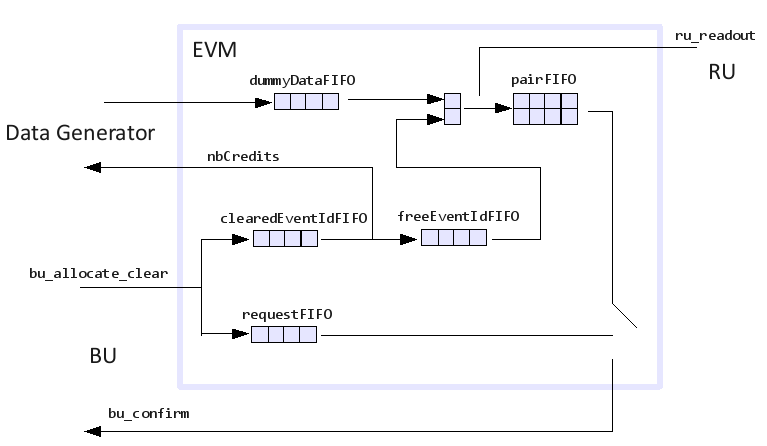
\includegraphics[width=0.90\textwidth]{figures/evm_behavior.png}
	\caption{Dynamic Behavior and Internal FIFOs of EVM}
	\label{fig:evm_behavior}
\end{figure}


\textbf{Step 1:} When the system is enabled the first event that the EVM receives is the $bu_allocate_clear$ event from the BU. Since there are no event requests available at the beginning, this event triggers the operation of the RU BUilder. Receipt of this event affects the $clearedEventId$ and $request$ FIFos of EVM. The incoming event may be for a new event id request, be a request for release of a used event id, or be a request for both release of a used event id and a request for new event id. Upon reciept of the event, appropriate FIFOs are filled.

At the same time, the initial request for event data is sent to the DataGenerator component. Along with the request, a parameter called $nbCredits$ is sent. This denotes the number of available free event id slots in the builder. In this first step, the number of available free event id's is the size of the freeEventIdFIFO. 

\textbf{Step 2:} If there were a request to release an event id in the previous step, the freeEventIdFIFO is populated with the released event id.

\textbf{Step 3:} EVM asks for new event data with the number of released event id's as $nbCredits$ from the DataGenerator.

\textbf{Step 4:} DataGenerator sends the generated dummy event data to the EVM. Upon receipt of the data, dummyDataFIFO is filled with the event data. 

\textbf{Step 5:} If dummyDataFIFO and freeEventIdFIFO is not empty then pairFIFO is filled with the free event id from the freeEventIdFIFO and the event number from the dummyDataFIFO.

\textbf{Step 6:} When the conditions for Step 5 are satisfied EVM also sends $ru_readout$ event to RU with the event id/event number pair. 

\textbf{Step 7:} If the requestFIFO is filled with a request from BU, and the pairFIFO is filled with a Event Id/Event Number, then EVM sends $bu_confirm$ event.

Figure \ref{fig:evmmodel1} shows the DEVS model of EVM with states and input and output events.

\begin{figure}
	\centering
		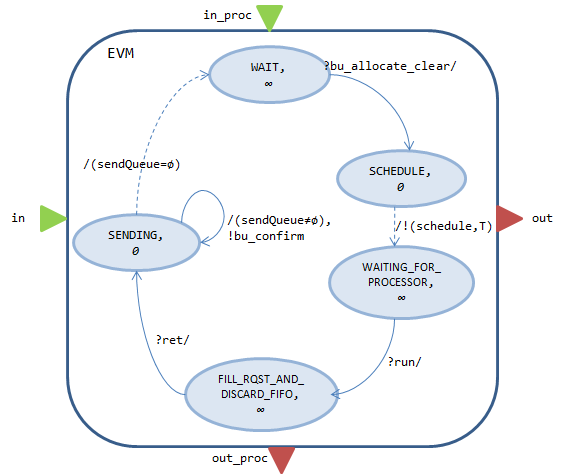
\includegraphics[width=0.95\textwidth]{figures/evmmodel1.png}
	\caption{EVM Model}
	\label{fig:evmmodel1}
\end{figure}

Initially, EVM is in WAIT state until an event is received. The events and state transition conditions are clearly indicated on the figure. EVM implements a queue called $sendQueue$ which is filled in when there is an output event to be sent out. 

\subsubsection{Readout Unit (RU)}
Readout unit is responsible for gathering the event data fragments and building super-fragments from them. Multiple fragments make up one complete event. DataGenerator generates dummy events with random fragment sizes. Figure \ref{fig:ru_behavior} shows the dynamic behavior of RU.

\begin{figure}
 \centering
 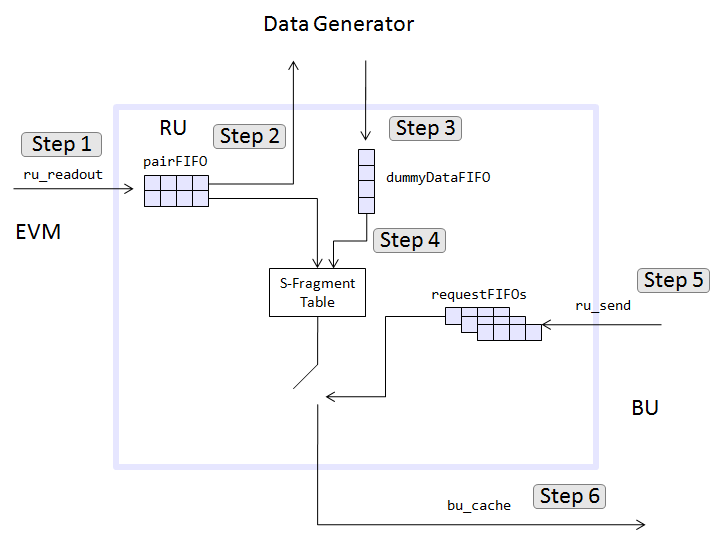
\includegraphics[width=0.90\textwidth]{figures/ru_behavior.png}
 % evm_behavior.png: 0x0 pixel, 0dpi, nanxnan cm, bb=
 \caption{Dynamic Behavior and Internal FIFOs of RU}
 \label{fig:ru_behavior}
\end{figure}


\textbf{Step 1:} The first step in the RU processing is the receipt of $ru_readout$ event from EVM. EVM sends RU a event id/event number pair for processing. RU populates its pairFIFO with event id/event number pair.

\textbf{Step 2:} RU asks the DataGenerator to send it the fragments of the event data that corresponds to the event number received from EVM.

\textbf{Step 3:} DataGenerator sends RU the number of blocks that  fragment for the specified event number is composed of. Upon reciept of the data the blockFIFO of RU is filled with the blocks received from the DataGenerator. In addition, at the same time, all blocks belonging to a single event are collected together to form event super-fragments.

\textbf{Step 4:} If the super-fragments are formed and pairFIFO is holding event id/event number pairs, then the table that is indexed by the event id from the pairFIFO and that holds all super-fragments is filled with super-fragment block.

\textbf{Step 5:} BU sends $ru_send$ event to request an event super-fragment to build. Upoxn reciept of the event, requestFIFO corresponding to the index of the BU that is requesting an event is populated.

\textbf{Step 6:} If any of the requestFIFOs is filled with a request, RU services the BU request with event super-fragments that are saved in the super-fragment table and sends out the $bu_cache$ event to BUs that requested an event.

Figure \ref{fig:rumodel1} shows the DEVS model of RU with states and input and output events.

\begin{figure}
	\centering
		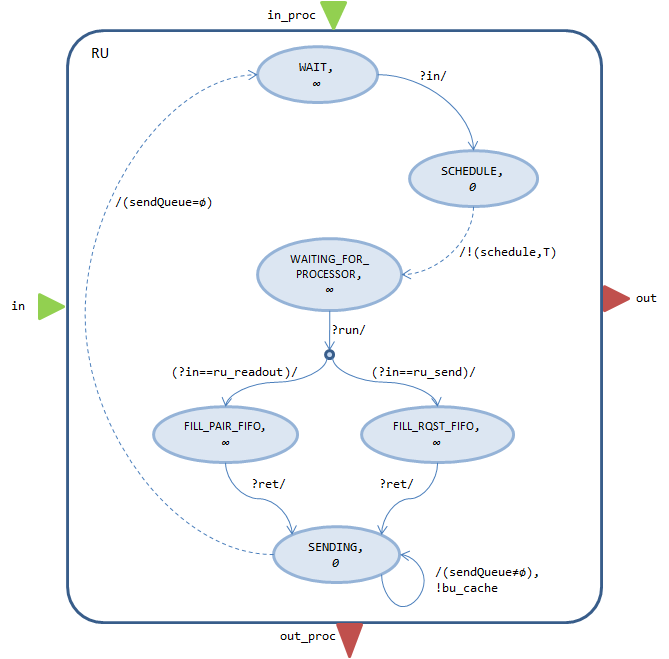
\includegraphics[width=0.95\textwidth]{figures/rumodel1.png}
	\caption{RU Model}
	\label{fig:rumodel1}
\end{figure}

\subsubsection{Builder Unit (BU)}
Builder Unit (BU) is responsible for building events  An event is composed of one super-fragment from coming from the DataGenerator and N RU super-fragments where N is the number of RUs. Figure \ref{fig:bu_behavior} shows the dynamic behavior of BU.

\begin{figure}
 \centering
 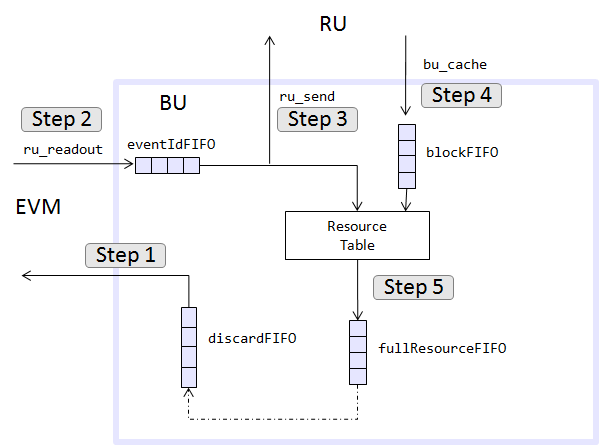
\includegraphics[width=0.90\textwidth]{figures/bu_behavior.png}
 % evm_behavior.png: 0x0 pixel, 0dpi, nanxnan cm, bb=
 \caption{Dynamic Behavior and Internal FIFOs of BU}
 \label{fig:bu_behavior}
\end{figure}


\textbf{Step 1:} As BU is enabled, the first action it takes is to send initial event requests to EVM. At this point the builder is completely available to build events. BU sends the event $bu_allocate_clear$ event to EVM.

\textbf{Step 2:} BU recieves the $bu_confirm$ event from EVM. Upon receipt of the event, BU fills in the eventIdFIFO with the id's of events that are assigned to the system by EVM. 

\textbf{Step 3:} If the eventIdFIFO is not empty, BU starts the construction of the event with the first event id in the eventIdFIFO and is ready to receive fragments of that event from RUs. At this point, BU sends out the $ru_send$ event to all RUs that are participating in the event building and asks for the fragments of the event that is under construction. Moreover, at this step, if a construction of an event is complete, then the fullResourceFIFO is filled by BU. This also increases the number of events built in the builder, and completes the lifecycle of an event id/event number pair.

\textbf{Step 4:} BU recieves the $bu_cache$ event from participating RUs. Upon receipt of this event, BU fills in the blockFIFO with blocks of event under construction.

\textbf{Step 5:} If there is an event data block in the blockFIFO then BU appends event block data to the previous blocks of the same event data. When  the event building is complete the number of events built in builder is incremented and the completed event block is put into the fullResourceFIFO. In addition, the completed event id ends its lifecycle and is pushed into the discardFIFO.

\textbf{Step 6:} In the simulation system, there is no Filter Unit to process the physical importance of those events. Instead the all the events are dropped after being completed and the number of events built in BU is incremented.

\textbf{Step 7:} If the discardFIFO is not empty then the used event id is recycled and $bu_allocate_clear$ is sent to EVM if the total number of events to be built has not been reached. 

Figure \ref{fig:bumodel1} shows the DEVS model of BU with states and input and output events. 


\begin{figure}
	\centering
		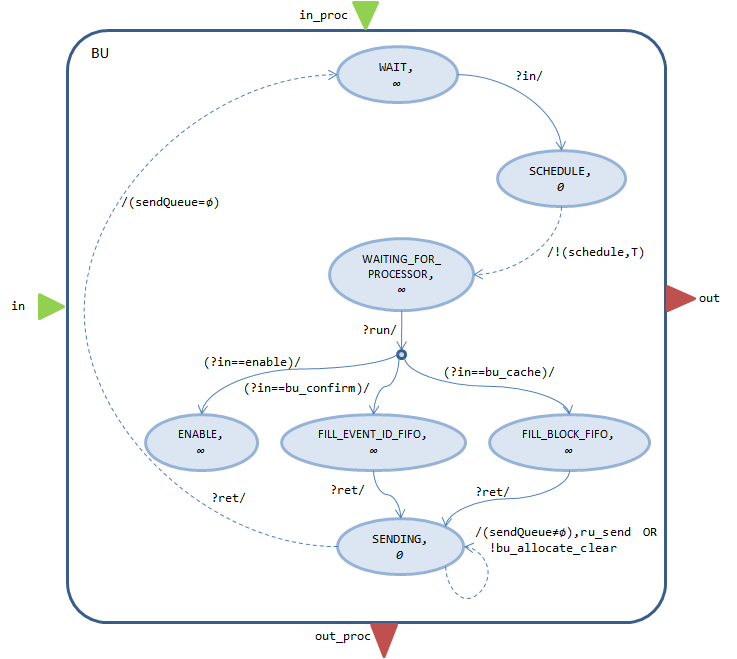
\includegraphics[width=0.95\textwidth]{figures/bumodel1.png}
	\caption{BU Model}
	\label{fig:bumodel1}
\end{figure}

\subsubsection{Peer Transport (PT)}
PeerTransport is the component that is responsible for transmitting messages between applications. Figure \ref{fig:pt_behavior} shows the dynamic behavior of the PeerTransport.

\begin{figure}
 \centering
 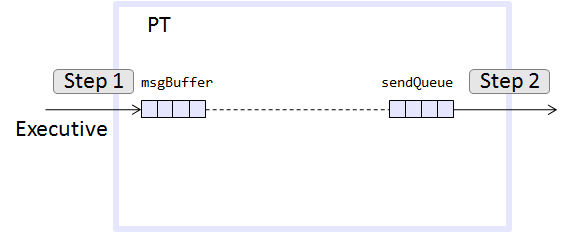
\includegraphics[width=0.90\textwidth]{figures/pt_behavior.png}
 % evm_behavior.png: 0x0 pixel, 0dpi, nanxnan cm, bb=
 \caption{Dynamic Behavior and Internal FIFOs of PT}
 \label{fig:pt_behavior}
\end{figure}

\textbf{Step 1:} PT receives $send$ event from the Executive. Upon receipt of the event, PT fills in the msgBufferFIFO. At this point, PT knows about the communication parties and the message that is being transmitted between them. 

\textbf{Step 2:} If the message buffer is not empty, PT puts the messages in the buffer into the sendQueueFIFO and sends out the message received from the Executive to all the applications. PT does not know the contents of the message or the event that is being transmitted. PT only transmits the message to all the applications and only the application with the id that matches the destination id of the message processes the event.

Figure \ref{fig:ptmodel1} shows the DEVS model of PT with states and input and output events.

\begin{figure}
	\centering
		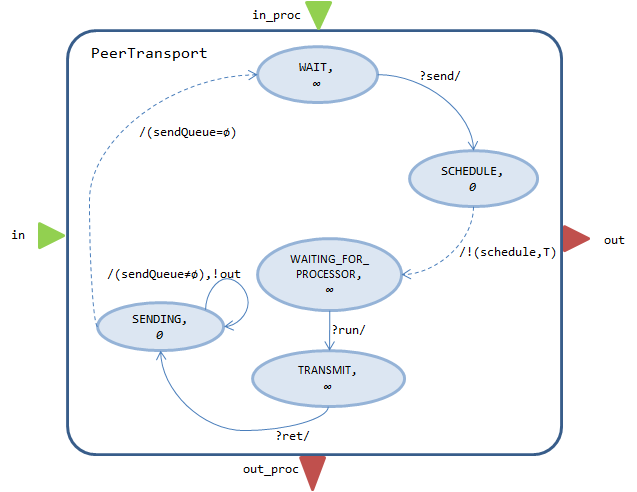
\includegraphics[width=0.95\textwidth]{figures/ptmodel1.png}
	\caption{PeerTransport Model}
	\label{fig:ptmodel1}
\end{figure}

\subsubsection{Executive}
Executive is the only application that resides in the middleware layer and is responsible with coordinating the communication of applications. Figure \ref{fig:executive_behavior} shows the dynamic behavior of the Executive.

\begin{figure}
 \centering
 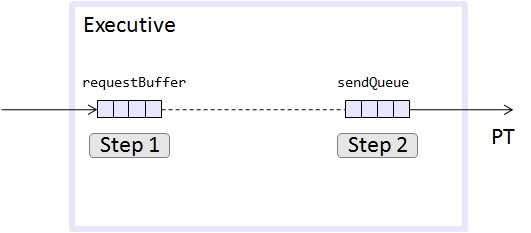
\includegraphics[width=0.90\textwidth]{figures/executive_behavior.png}
 % evm_behavior.png: 0x0 pixel, 0dpi, nanxnan cm, bb=
 \caption{Dynamic Behavior and Internal FIFOs of Executive}
 \label{fig:executive_behavior}
\end{figure}

\textbf{Step 1:} An application that needs to send an event to another application sends the event to the Executive. Upon receipt of the message from any application on its input port, the Executive saves the message into the requestBufferFIFO. 

\textbf{Step 2:} Executive knows about the available PeerTransports to use to send messages to the desired applications. Executive sends the $send$ event to the appropriate PT. 

Figure \ref{fig:executivemodel1} shows the DEVS model of Executive with states and input and output events. 

\begin{figure}
	\centering
		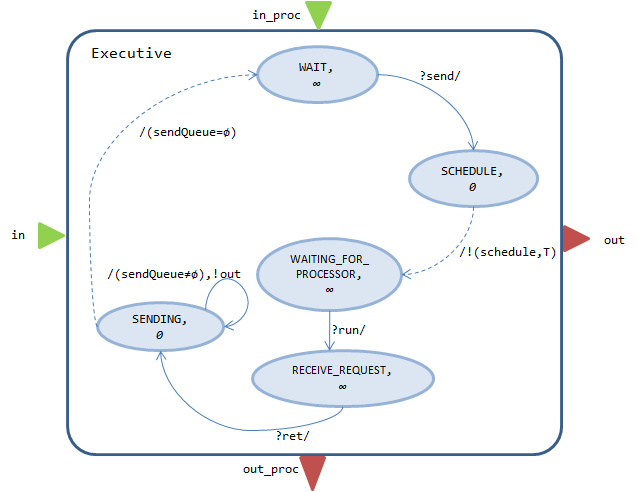
\includegraphics[width=0.95\textwidth]{figures/executivemodel1.png}
	\caption{Executive Model}
	\label{fig:executivemodel1}
\end{figure}

\subsection{Processor Model}
The experimental framework also includes a processor model to implement simple scheduling. Figure \ref{fig:Processor} shows the DEVS model of the processor along with it states, transition conditions and inputs and outputs.


\begin{figure}
	\centering
		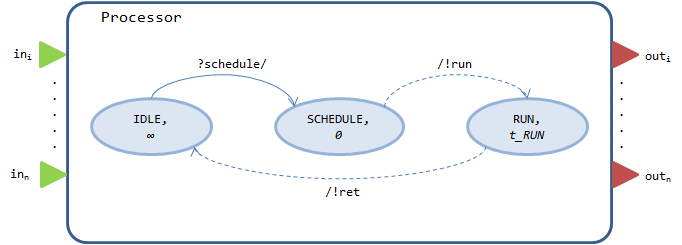
\includegraphics[width=0.99\textwidth]{figures/Processor.png}
	\caption{Processor DEVS Model}
	\label{fig:Processor}
\end{figure}

Processor receives a scheduling request from an application. Along with the scheduling request, application also sends the time it requests. The processor buffers all the scheduling requests. Then the ``$run$'' event is sent to the requesting application while the processor switches from the IDLE state to the RUN state. The life span of the RUN state of the processor becomes the amount of time requested by the application. Once the lifespan of the RUN state is elapsed, processor sends out the ``$ret$'' event to ask the application to return. Processor has several input and output ports. Every application has an input port connecting it to the processor, and there is one output port for every application to connect the processor output to the applications.


!!!PUT AN IMAGE OF THE SYSTEM!!!

\section{Performance Aspect in Models}
DEVS models of applications are given in the previous sections. It's also important to note that some parameters related to the performance of the system are also captured in the application models. These parameters are mainly parameters of RU Builder applications. 

The XDAQ system is distributed as a software package by CERN which does not allow tuning of performance or modification of any performance related parameters. The tuning is done by the developers for only the case for which the system is going to be deployed for the experiment. However, for the purposes of this research, it was crucial to know the parameters which are highly probable to have an impact on the system performance. 

Upon conversations with XDAQ developers, it was made clear that so called packing parameters, and total number of blocks that make up a s-fragment are among the most important parameters that affect the performance of the system. In the original XDAQ system all packing parameters are set as $8$. Fragment sizes change during operation as different events have differing amounts of data. 

Packing parameters are captured in EVM and BU models. EVM has \textit{RU\_READOUT\_PACKING} parameter which determines how many requests need to be packed before sending a readout request to RUs. BU has \textit{EVM\_ALLOCATE\_CLEAR\_PACKING} which determines how many requests need to be packed before requesting or releasing an event id  and \textit{RU\_SEND\_PACKING} which determines how many requests need to be packed before sending s-fragment requests from RUs.

In addition to the packing parameters, BU model captures $blockFIFOCapacity$, $requestFIFOCapacity$, and $maxEvtsUnderConstruction$ which determines the maximum number of events that can be constructed in BU.

Differing event data block sizes are not captured in the application models but rather in the data generator which is explained in the next section. 

\section{Data Generation}
In order to drive the experiment platform and the simulation, a dummy input data generator is needed. As stated in the previous section, differing event data fragment sizes are generated by the dummy data generator and fed into the system. 

Number of blocks in s-fragment is a statical distribution since different events have different amounts of data. This is captured in the data generator by use of a random number generator using a normal distribution. Boost Random library is used with a Mersenne Twister random number generator with normal distribution \cite{boost}. Data generator is not a DEVS model. 


\section{Communication Interfaces Between Applications}

\subsection{EVM-BU Interface}

EVM and BU has two way interface. Figure \ref{fig:evm-bu} shows the events passed between EVM and BU.
\begin{figure}
	\centering
		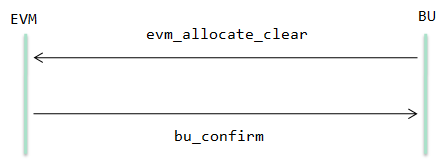
\includegraphics[width=0.85\textwidth]{figures/evm-bu.png}
	\caption{EVM-BU Interface Diagram}
	\label{fig:evm-bu}
\end{figure}

BU starts the interaction between itself and EVM by sending event requests by sending the \textit{evm\_allocate\_clear}. The message format of the communication between EVM and BU is as follows: 
\begin{quote}
	address\#sourceId\#destinationId\#event\#data
\end{quote}

BU sends the following data along with the event:

\begin{itemize}
	\item \textbf{buAddress}: The IP address of the computer that the BU is running on
	\item \textbf{buId}: Unique identifier of the source application, BU
	\item \textbf{destinationId}: Unique identifier of the destination application
	\item \textbf{eventName}: Name of the event which is \textit{evm\_allocate\_clear} in this case
	\item \textbf{data}: Actual request message which consists of the request.
\end{itemize}

In order to form the request data, BU sets the following parameters:
\begin{itemize}
	\item BU Id: The unique identifier of the BU that is making the request.
	\item Number of Requests Packed: BU does not send one request at a time but packs multiple requests into one request. The total number of requests are sent as part of the request data.
	\item Request type: $0$ means event id request, $1$ means releasing an event id and requesting another, and $2$ means releasing an event id.
	\item Event Id: Event id to be released. If requesting an id, this is not need to be set.
	\item Event Number: Event number that is associated with the released event id. If requesting an id, this is not need to be set.
	\item Resource Id: The resource id of the BU that is making the request.
\end{itemize}

EVM receives the request from the BU and acts on it. As a result, EVM sends out the \textit{bu\_confirm} event to the requesting BU. EVM sends the following data along with the event:

\begin{itemize}
	\item \textbf{evmAddress}: The IP address of the computer that the EVM is running on
	\item \textbf{evmId}: Unique identifier of the source application, EVM
	\item \textbf{buId}: Unique identifier of the destination application, BU
	\item \textbf{event}: Name of the event which is \textit{bu\_confirm} in this case
	\item \textbf{data}: The confirmation message to BU
\end{itemize}

In order to for the confirmation data, EVM sets the following parameters:

\begin{itemize}
	\item \textbf{Event Number (eventNumber)}: Event number assigned to BU
	\item \textbf{Number of Blocks In Superfragment (nbBlocksInSuperFragment)}: Number of blocks that make up the sfragment
	\item \textbf{Block Number (blockNb)}: The position of the current block in the sfragment. It is set as $0$ at this time.
	\item \textbf{Event Id (eventId)}: Event id that is assigned to the BU.
	\item \textbf{Superfragment Number (superFragmentNb)}: The number of the superfragment in the block. Set as $0$ for the first set of data.
\end{itemize}


\subsection{EVM-RU Interface}

EVM and RU has a one way interface. Figure \ref{fig:evm-ru} shows the interaction between EVM and RU.

\begin{figure}
	\centering
		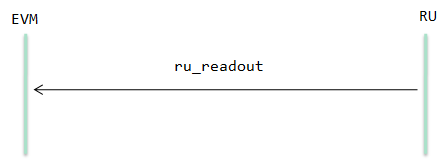
\includegraphics[width=0.85\textwidth]{figures/evm-ru.png}
	\caption{EVM-RU Interface Diagram}
	\label{fig:evm-ru}
\end{figure}

EVM sends RUs the \textit{readout} event. The message format of the communication between EVM and RU is as follows:

\begin{quote}
	address\#sourceId\#destinationId\#event\#data
\end{quote}

EVM sends the following data along with the event:

\begin{itemize}
	\item \textbf{Number of Elements Packed}: Total number of read out requests that is packed. EVM doesn't send events one by one. Multiple read out requests are sent.
	\item \textbf{Event Id}: Event id to be read out from the data generator.
	\item \textbf{Event Number}: Event number of the data that is read out from the data generator.
\end{itemize}


\subsection{BU-RU Interface}

BU and RU has a two way interface. Figure \ref{fig:bu-ru} shows the interaction between BU and RU.

\begin{figure}
	\centering
		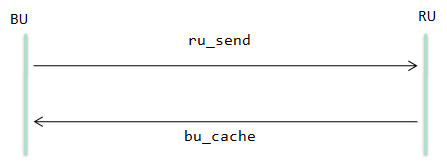
\includegraphics[width=0.85\textwidth]{figures/bu-ru.png}
	\caption{BU-RU Interface Diagram}
	\label{fig:bu-ru}
\end{figure}

The message format of the communication is as follows:

\begin{quote}
	address\#sourceId\#destinationId\#event\#data
\end{quote}

BU sends RU the \textit{ru\_send} event. BU sends the following data along with the event:

\begin{itemize}
	\item \textbf{Event Id}: Event id of the event that BU is requesting
	\item \textbf{Event Number}: Event number of the event that BU is requesting
	\item \textbf{BU Resource Id}: Resource id of the BU that is going to build the event
	\item \textbf{BU Id}: Unique identifier of BU that is requesting the event data
\end{itemize}

RU sends BU the ''\textit{bu\_cache}'' event. RU sends the following data along with the event:

\begin{itemize}
	\item \textbf{Block Number}: The current block number of the event data in the data chain
	\item	\textbf{BU Resource Id}: Resource id of the BU that is going to build the event
	\item \textbf{Event Id}: Event id of the event that BU is requesting
	\item \textbf{Event Number}: Event number of the evet that BU is requesting
	\item \textbf{Number of Blocks in Superfragment}: Total number of blocks that make up the s-fragment
	\item \textbf{Superfragment Number}: The current s-fragment number in the s-fragment chain
\end{itemize}


\subsection{Application-Executive-PT Interface}

The Executive has one way interface with all the applications. Figure \ref{fig:exec-pt} shows the interaction between applications, executive, and peer transport.

\begin{figure}
	\centering
		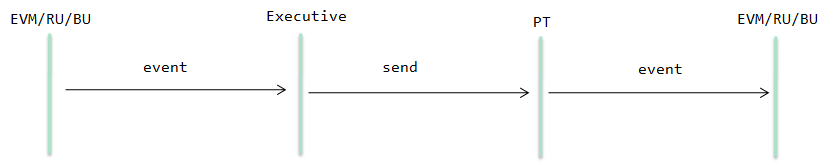
\includegraphics[width=1.0\textwidth]{figures/exec-pt.png}
	\caption{Executive-Peer Transport Interface Diagram}
	\label{fig:exec-pt}
\end{figure}

Since applications need to go through the Executive to pass data to other applications, the above mentioned communication should go through the Executive. 

Executive sends PT the \textit{send} event. The message format is the same as given above since Executive does not need any extra information and transmit the data without making any modifications to it. Executive sends the data received from the application along with the event. 

PT has one way interface with the the applications. PT sends the destination application the original event that is being transmitted between the applications. PT does not also make any modifications to the data being transmitted.



\subsection{Application-Processor Interface}

Processor has two-way interface with all the applications. All applications go through the Processor for scheduling processing time. Figure \ref{fig:processor-app} shows the interaction between applications and the Processor.

\begin{figure}
	\centering
		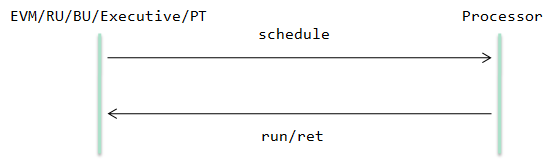
\includegraphics[width=0.85\textwidth]{figures/processor-app.png}
	\caption{Processor-Application Interface}
	\label{fig:processor-app}
\end{figure}

Applications send the Processor the \textit{schedule} event when they request scheduling. Applications send the requested amount of time along with the event.

Processor sends the requesting application the \textit{run} event to notify it to start running. Processor does not pass any data along with the event.

Processor sends the scheduled application the \textit{ret} event to notify that the time is up and the application should return. Processor does not pass any data along with the event. 


\section{Summary}
****TODO****


